\documentclass[twoside]{book}

% Packages required by doxygen
\usepackage{fixltx2e}
\usepackage{calc}
\usepackage{doxygen}
\usepackage[export]{adjustbox} % also loads graphicx
\usepackage{graphicx}
\usepackage[utf8]{inputenc}
\usepackage{makeidx}
\usepackage{multicol}
\usepackage{multirow}
\PassOptionsToPackage{warn}{textcomp}
\usepackage{textcomp}
\usepackage[nointegrals]{wasysym}
\usepackage[table]{xcolor}

% Font selection
\usepackage[T1]{fontenc}
\usepackage[scaled=.90]{helvet}
\usepackage{courier}
\usepackage{amssymb}
\usepackage{sectsty}
\renewcommand{\familydefault}{\sfdefault}
\allsectionsfont{%
  \fontseries{bc}\selectfont%
  \color{darkgray}%
}
\renewcommand{\DoxyLabelFont}{%
  \fontseries{bc}\selectfont%
  \color{darkgray}%
}
\newcommand{\+}{\discretionary{\mbox{\scriptsize$\hookleftarrow$}}{}{}}

% Page & text layout
\usepackage{geometry}
\geometry{%
  a4paper,%
  top=2.5cm,%
  bottom=2.5cm,%
  left=2.5cm,%
  right=2.5cm%
}
\tolerance=750
\hfuzz=15pt
\hbadness=750
\setlength{\emergencystretch}{15pt}
\setlength{\parindent}{0cm}
\setlength{\parskip}{3ex plus 2ex minus 2ex}
\makeatletter
\renewcommand{\paragraph}{%
  \@startsection{paragraph}{4}{0ex}{-1.0ex}{1.0ex}{%
    \normalfont\normalsize\bfseries\SS@parafont%
  }%
}
\renewcommand{\subparagraph}{%
  \@startsection{subparagraph}{5}{0ex}{-1.0ex}{1.0ex}{%
    \normalfont\normalsize\bfseries\SS@subparafont%
  }%
}
\makeatother

% Headers & footers
\usepackage{fancyhdr}
\pagestyle{fancyplain}
\fancyhead[LE]{\fancyplain{}{\bfseries\thepage}}
\fancyhead[CE]{\fancyplain{}{}}
\fancyhead[RE]{\fancyplain{}{\bfseries\leftmark}}
\fancyhead[LO]{\fancyplain{}{\bfseries\rightmark}}
\fancyhead[CO]{\fancyplain{}{}}
\fancyhead[RO]{\fancyplain{}{\bfseries\thepage}}
\fancyfoot[LE]{\fancyplain{}{}}
\fancyfoot[CE]{\fancyplain{}{}}
\fancyfoot[RE]{\fancyplain{}{\bfseries\scriptsize Generated by Doxygen }}
\fancyfoot[LO]{\fancyplain{}{\bfseries\scriptsize Generated by Doxygen }}
\fancyfoot[CO]{\fancyplain{}{}}
\fancyfoot[RO]{\fancyplain{}{}}
\renewcommand{\footrulewidth}{0.4pt}
\renewcommand{\chaptermark}[1]{%
  \markboth{#1}{}%
}
\renewcommand{\sectionmark}[1]{%
  \markright{\thesection\ #1}%
}

% Indices & bibliography
\usepackage{natbib}
\usepackage[titles]{tocloft}
\setcounter{tocdepth}{3}
\setcounter{secnumdepth}{5}
\makeindex

% Hyperlinks (required, but should be loaded last)
\usepackage{ifpdf}
\ifpdf
  \usepackage[pdftex,pagebackref=true]{hyperref}
\else
  \usepackage[ps2pdf,pagebackref=true]{hyperref}
\fi
\hypersetup{%
  colorlinks=true,%
  linkcolor=blue,%
  citecolor=blue,%
  unicode%
}

% Custom commands
\newcommand{\clearemptydoublepage}{%
  \newpage{\pagestyle{empty}\cleardoublepage}%
}

\usepackage{caption}
\captionsetup{labelsep=space,justification=centering,font={bf},singlelinecheck=off,skip=4pt,position=top}

%===== C O N T E N T S =====

\begin{document}

% Titlepage & ToC
\hypersetup{pageanchor=false,
             bookmarksnumbered=true,
             pdfencoding=unicode
            }
\pagenumbering{roman}
\begin{titlepage}
\vspace*{7cm}
\begin{center}%
{\Large P\+D\+A\+RT }\\
\vspace*{1cm}
{\large Generated by Doxygen 1.8.11}\\
\end{center}
\end{titlepage}
\clearemptydoublepage
\tableofcontents
\clearemptydoublepage
\pagenumbering{arabic}
\hypersetup{pageanchor=true}

%--- Begin generated contents ---
\chapter{Hierarchical Index}
\section{Class Hierarchy}
This inheritance list is sorted roughly, but not completely, alphabetically\+:\begin{DoxyCompactList}
\item Q\+Dialog\begin{DoxyCompactList}
\item \contentsline{section}{New\+Shape\+Model\+Dialog}{\pageref{class_new_shape_model_dialog}}{}
\item \contentsline{section}{Selected\+Point\+Widget}{\pageref{class_selected_point_widget}}{}
\end{DoxyCompactList}
\item Q\+Main\+Window\begin{DoxyCompactList}
\item \contentsline{section}{Main\+Window}{\pageref{class_main_window}}{}
\end{DoxyCompactList}
\item vtk\+Area\+Picker\begin{DoxyCompactList}
\item \contentsline{section}{Inherited\+Picker}{\pageref{class_inherited_picker}}{}
\end{DoxyCompactList}
\item vtk\+Interactor\+Style\+Rubber\+Band\+Pick\begin{DoxyCompactList}
\item \contentsline{section}{Interactor\+Style}{\pageref{class_interactor_style}}{}
\end{DoxyCompactList}
\end{DoxyCompactList}

\chapter{Class Index}
\section{Class List}
Here are the classes, structs, unions and interfaces with brief descriptions\+:\begin{DoxyCompactList}
\item\contentsline{section}{\hyperlink{class_inherited_picker}{Inherited\+Picker} }{\pageref{class_inherited_picker}}{}
\item\contentsline{section}{\hyperlink{class_interactor_style}{Interactor\+Style} }{\pageref{class_interactor_style}}{}
\item\contentsline{section}{\hyperlink{class_main_window}{Main\+Window} }{\pageref{class_main_window}}{}
\item\contentsline{section}{\hyperlink{class_new_shape_model_dialog}{New\+Shape\+Model\+Dialog} }{\pageref{class_new_shape_model_dialog}}{}
\item\contentsline{section}{\hyperlink{class_selected_point_widget}{Selected\+Point\+Widget} }{\pageref{class_selected_point_widget}}{}
\end{DoxyCompactList}

\chapter{Class Documentation}
\hypertarget{class_inherited_picker}{}\section{Inherited\+Picker Class Reference}
\label{class_inherited_picker}\index{Inherited\+Picker@{Inherited\+Picker}}


{\ttfamily \#include $<$Inherited\+Picker.\+h$>$}

Inheritance diagram for Inherited\+Picker\+:\begin{figure}[H]
\begin{center}
\leavevmode
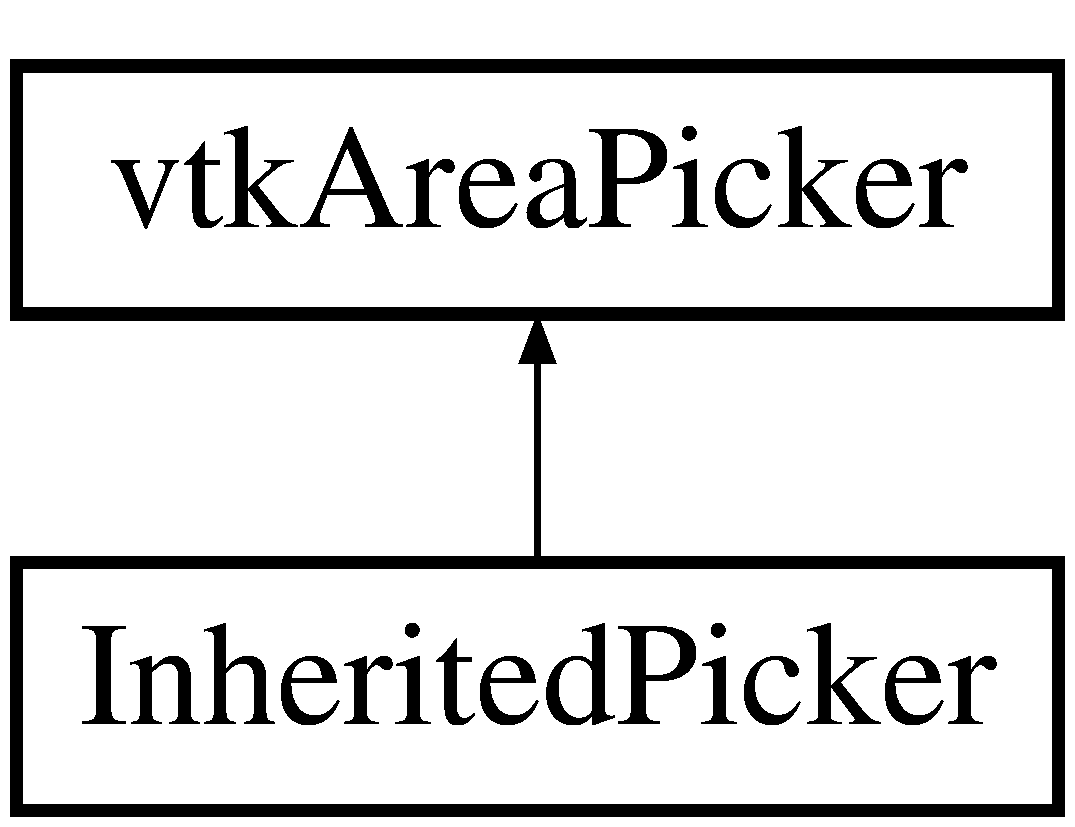
\includegraphics[height=2.000000cm]{class_inherited_picker}
\end{center}
\end{figure}
\subsection*{Public Member Functions}
\begin{DoxyCompactItemize}
\item 
int {\bfseries get\+\_\+\+X0} ()\hypertarget{class_inherited_picker_a43ed269bda4a7b27dc3f5fbb7c3da776}{}\label{class_inherited_picker_a43ed269bda4a7b27dc3f5fbb7c3da776}

\item 
int {\bfseries get\+\_\+\+X1} ()\hypertarget{class_inherited_picker_aed9b3615fc071c5c5e5a644e8e93bfc8}{}\label{class_inherited_picker_aed9b3615fc071c5c5e5a644e8e93bfc8}

\item 
int {\bfseries get\+\_\+\+Y0} ()\hypertarget{class_inherited_picker_a8c110b15b43d402965565b60bd8f327e}{}\label{class_inherited_picker_a8c110b15b43d402965565b60bd8f327e}

\item 
int {\bfseries get\+\_\+\+Y1} ()\hypertarget{class_inherited_picker_a9a37a7b8a9a0cbda4c636540706ae5df}{}\label{class_inherited_picker_a9a37a7b8a9a0cbda4c636540706ae5df}

\item 
std\+::vector$<$ int $>$ {\bfseries get\+\_\+dimensions} ()\hypertarget{class_inherited_picker_a01513df00a5a7677525f5c8ff6b15c68}{}\label{class_inherited_picker_a01513df00a5a7677525f5c8ff6b15c68}

\end{DoxyCompactItemize}


\subsection{Detailed Description}
Definition of the \hyperlink{class_inherited_picker}{Inherited\+Picker} class. This class directly inherits from vtk\+Area\+Picker. Used as an interface that allows the user to get access to the dimensions of the picking area. 

The documentation for this class was generated from the following file\+:\begin{DoxyCompactItemize}
\item 
pdart\+\_\+prototype/source/Inherited\+Picker.\+h\end{DoxyCompactItemize}

\hypertarget{class_interactor_style}{}\section{Interactor\+Style Class Reference}
\label{class_interactor_style}\index{Interactor\+Style@{Interactor\+Style}}


{\ttfamily \#include $<$Interactor.\+h$>$}

Inheritance diagram for Interactor\+Style\+:\begin{figure}[H]
\begin{center}
\leavevmode
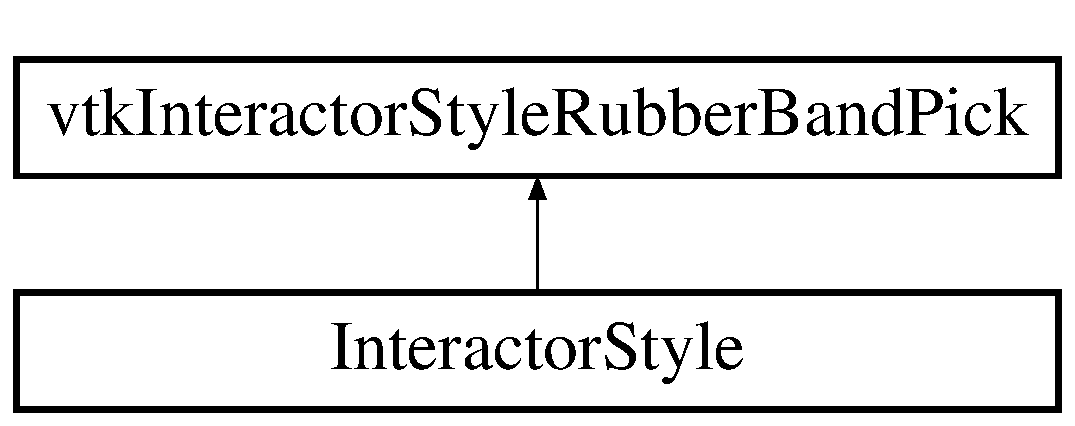
\includegraphics[height=2.000000cm]{class_interactor_style}
\end{center}
\end{figure}
\subsection*{Public Member Functions}
\begin{DoxyCompactItemize}
\item 
{\bfseries vtk\+Type\+Macro} (\hyperlink{class_interactor_style}{Interactor\+Style}, vtk\+Interactor\+Style\+Rubber\+Band\+Pick)\hypertarget{class_interactor_style_a43338f1434b768677a2feac0b1a05c13}{}\label{class_interactor_style_a43338f1434b768677a2feac0b1a05c13}

\item 
virtual void {\bfseries On\+Left\+Button\+Up} ()\hypertarget{class_interactor_style_a441fa7b70b39c61768f0d9a8d48faf3c}{}\label{class_interactor_style_a441fa7b70b39c61768f0d9a8d48faf3c}

\item 
void \hyperlink{class_interactor_style_aca72fd8ef4db10f2356795ae9cf32d9b}{Set\+Points} (vtk\+Smart\+Pointer$<$ vtk\+Poly\+Data $>$ points\+\_\+polydata)
\item 
void \hyperlink{class_interactor_style_aa7d59db5ac179da9469081c14e77b6d0}{Set\+Main\+Window} (\hyperlink{class_main_window}{Main\+Window} $\ast$mainwindow)
\end{DoxyCompactItemize}
\subsection*{Static Public Member Functions}
\begin{DoxyCompactItemize}
\item 
static \hyperlink{class_interactor_style}{Interactor\+Style} $\ast$ {\bfseries New} ()\hypertarget{class_interactor_style_aaea3b0cff00feb99c42325bf49168fc6}{}\label{class_interactor_style_aaea3b0cff00feb99c42325bf49168fc6}

\end{DoxyCompactItemize}


\subsection{Detailed Description}
Declaration of the \hyperlink{class_interactor_style}{Interactor\+Style}. This class enables the user to access (read A\+ND write) the underlying data displayed in the Q\+V\+T\+K\+Widget of the main window 

\subsection{Member Function Documentation}
\index{Interactor\+Style@{Interactor\+Style}!Set\+Main\+Window@{Set\+Main\+Window}}
\index{Set\+Main\+Window@{Set\+Main\+Window}!Interactor\+Style@{Interactor\+Style}}
\subsubsection[{\texorpdfstring{Set\+Main\+Window(\+Main\+Window $\ast$mainwindow)}{SetMainWindow(MainWindow *mainwindow)}}]{\setlength{\rightskip}{0pt plus 5cm}void Interactor\+Style\+::\+Set\+Main\+Window (
\begin{DoxyParamCaption}
\item[{{\bf Main\+Window} $\ast$}]{mainwindow}
\end{DoxyParamCaption}
)}\hypertarget{class_interactor_style_aa7d59db5ac179da9469081c14e77b6d0}{}\label{class_interactor_style_aa7d59db5ac179da9469081c14e77b6d0}
Enables the interactor to get access to the G\+UI\textquotesingle{}s mainwindow 
\begin{DoxyParams}{Parameters}
{\em points\+\_\+polydata} & Pointer to the G\+UI\textquotesingle{}s mainwindow \\
\hline
\end{DoxyParams}
\index{Interactor\+Style@{Interactor\+Style}!Set\+Points@{Set\+Points}}
\index{Set\+Points@{Set\+Points}!Interactor\+Style@{Interactor\+Style}}
\subsubsection[{\texorpdfstring{Set\+Points(vtk\+Smart\+Pointer$<$ vtk\+Poly\+Data $>$ points\+\_\+polydata)}{SetPoints(vtkSmartPointer< vtkPolyData > points_polydata)}}]{\setlength{\rightskip}{0pt plus 5cm}void Interactor\+Style\+::\+Set\+Points (
\begin{DoxyParamCaption}
\item[{vtk\+Smart\+Pointer$<$ vtk\+Poly\+Data $>$}]{points\+\_\+polydata}
\end{DoxyParamCaption}
)}\hypertarget{class_interactor_style_aca72fd8ef4db10f2356795ae9cf32d9b}{}\label{class_interactor_style_aca72fd8ef4db10f2356795ae9cf32d9b}
Enables the interactor to get access to the vtk\+Poly\+Data storing the shape\textquotesingle{}s vertices 
\begin{DoxyParams}{Parameters}
{\em points\+\_\+polydata} & Pointer to the vtk\+Poly\+Data storing the vertices of the shape model \\
\hline
\end{DoxyParams}


The documentation for this class was generated from the following files\+:\begin{DoxyCompactItemize}
\item 
pdart\+\_\+prototype/source/Interactor.\+h\item 
pdart\+\_\+prototype/source/Interactor.\+cpp\end{DoxyCompactItemize}

\hypertarget{class_main_window}{}\section{Main\+Window Class Reference}
\label{class_main_window}\index{Main\+Window@{Main\+Window}}


{\ttfamily \#include $<$mainwindow.\+h$>$}

Inheritance diagram for Main\+Window\+:\begin{figure}[H]
\begin{center}
\leavevmode
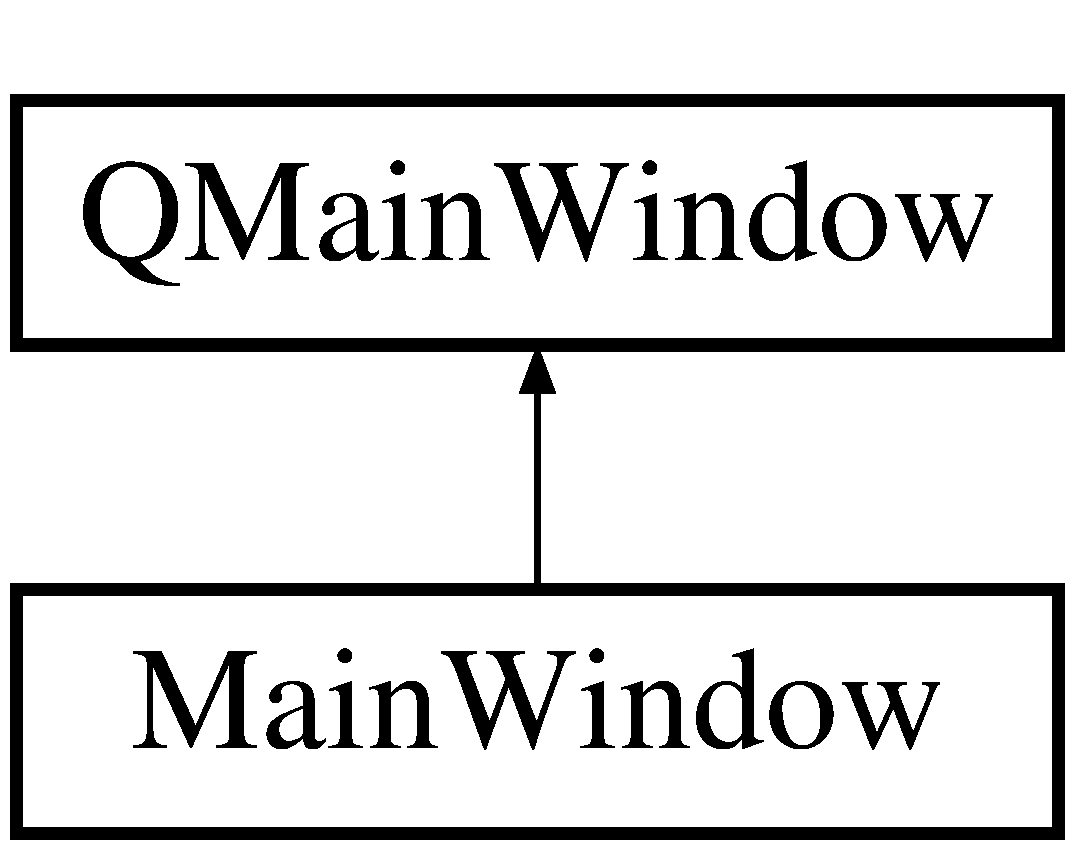
\includegraphics[height=2.000000cm]{class_main_window}
\end{center}
\end{figure}
\subsection*{Public Member Functions}
\begin{DoxyCompactItemize}
\item 
vtk\+Smart\+Pointer$<$ vtk\+Renderer $>$ \hyperlink{class_main_window_a2fb384b2232488ced24aad4237e0290e}{get\+Renderer} ()
\item 
\hyperlink{class_main_window_a34c4b4207b46d11a4100c9b19f0e81bb}{Main\+Window} ()
\end{DoxyCompactItemize}
\subsection*{Public Attributes}
\begin{DoxyCompactItemize}
\item 
Q\+V\+T\+K\+Widget $\ast$ {\bfseries qvtk\+Widget}\hypertarget{class_main_window_a987c16edfdf86679ea180e3c1af08e07}{}\label{class_main_window_a987c16edfdf86679ea180e3c1af08e07}

\item 
Q\+Widget $\ast$ {\bfseries central\+\_\+wrapping\+\_\+widget}\hypertarget{class_main_window_a607a0ae3a2d1785d11b65560e125f835}{}\label{class_main_window_a607a0ae3a2d1785d11b65560e125f835}

\item 
Q\+Widget $\ast$ {\bfseries dock\+\_\+wrapping\+\_\+widget}\hypertarget{class_main_window_a867cba72789a67607c2029391cb29b6b}{}\label{class_main_window_a867cba72789a67607c2029391cb29b6b}

\item 
Q\+H\+Box\+Layout $\ast$ {\bfseries layout\+\_\+central}\hypertarget{class_main_window_a6c85c0aeb8404eb5f0bb5b9a8a640d0f}{}\label{class_main_window_a6c85c0aeb8404eb5f0bb5b9a8a640d0f}

\item 
Q\+V\+Box\+Layout $\ast$ {\bfseries layout\+\_\+dock\+\_\+right}\hypertarget{class_main_window_af64854e3c836aa6ad4e8d85e553dd58e}{}\label{class_main_window_af64854e3c836aa6ad4e8d85e553dd58e}

\item 
Q\+Dock\+Widget $\ast$ {\bfseries menu\+\_\+dock}\hypertarget{class_main_window_a2e7fc292c9a123fd522a363844e39fa0}{}\label{class_main_window_a2e7fc292c9a123fd522a363844e39fa0}

\item 
bool {\bfseries selector\+Active} = false\hypertarget{class_main_window_a330930fdef1adf6db5446c93e203c9b2}{}\label{class_main_window_a330930fdef1adf6db5446c93e203c9b2}

\end{DoxyCompactItemize}


\subsection{Detailed Description}
Declaration of the \hyperlink{class_main_window}{Main\+Window} Class. Main class of the G\+UI as it hosts the V\+TK pipeline visualizer and the actions/menus allowing the user to interact with the program data. 

\subsection{Constructor \& Destructor Documentation}
\index{Main\+Window@{Main\+Window}!Main\+Window@{Main\+Window}}
\index{Main\+Window@{Main\+Window}!Main\+Window@{Main\+Window}}
\subsubsection[{\texorpdfstring{Main\+Window()}{MainWindow()}}]{\setlength{\rightskip}{0pt plus 5cm}Main\+Window\+::\+Main\+Window (
\begin{DoxyParamCaption}
{}
\end{DoxyParamCaption}
)}\hypertarget{class_main_window_a34c4b4207b46d11a4100c9b19f0e81bb}{}\label{class_main_window_a34c4b4207b46d11a4100c9b19f0e81bb}
Constructor. Setups the G\+UI and creates an instance of Q\+V\+TK Widget 

\subsection{Member Function Documentation}
\index{Main\+Window@{Main\+Window}!get\+Renderer@{get\+Renderer}}
\index{get\+Renderer@{get\+Renderer}!Main\+Window@{Main\+Window}}
\subsubsection[{\texorpdfstring{get\+Renderer()}{getRenderer()}}]{\setlength{\rightskip}{0pt plus 5cm}vtk\+Smart\+Pointer$<$ vtk\+Renderer $>$ Main\+Window\+::get\+Renderer (
\begin{DoxyParamCaption}
{}
\end{DoxyParamCaption}
)}\hypertarget{class_main_window_a2fb384b2232488ced24aad4237e0290e}{}\label{class_main_window_a2fb384b2232488ced24aad4237e0290e}
Returns a pointer to the vtk\+Renderer associated with the window\textquotesingle{}s Q\+V\+TK widget \begin{DoxyReturn}{Returns}
Pointer to the vtk\+Renderer associated with the window\textquotesingle{}s Q\+V\+TK widget 
\end{DoxyReturn}


The documentation for this class was generated from the following files\+:\begin{DoxyCompactItemize}
\item 
pdart\+\_\+prototype/source/mainwindow.\+h\item 
pdart\+\_\+prototype/source/mainwindow.\+cpp\end{DoxyCompactItemize}

\hypertarget{class_new_shape_model_dialog}{}\section{New\+Shape\+Model\+Dialog Class Reference}
\label{class_new_shape_model_dialog}\index{New\+Shape\+Model\+Dialog@{New\+Shape\+Model\+Dialog}}


{\ttfamily \#include $<$newshapemodeldialog.\+h$>$}

Inheritance diagram for New\+Shape\+Model\+Dialog\+:\begin{figure}[H]
\begin{center}
\leavevmode
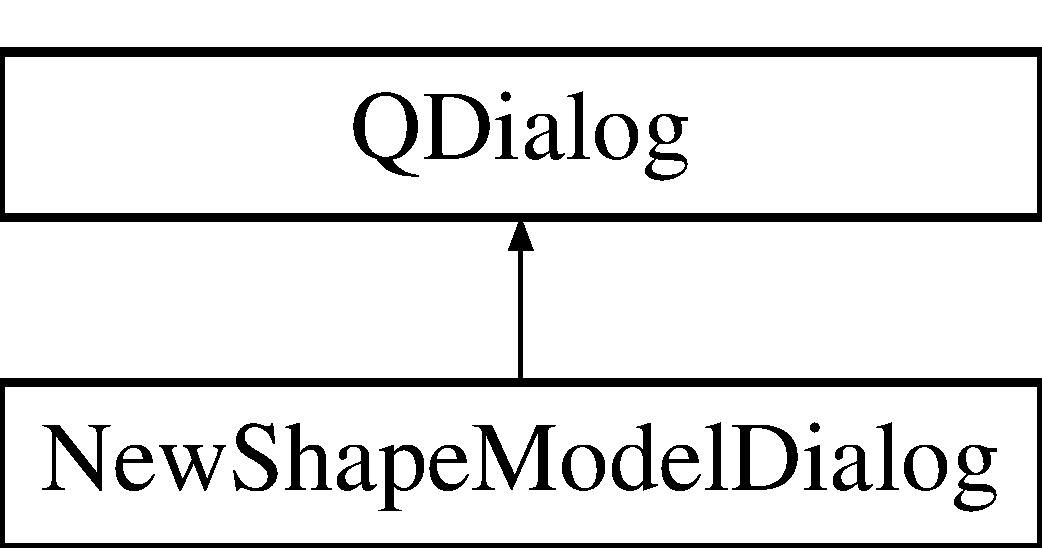
\includegraphics[height=2.000000cm]{class_new_shape_model_dialog}
\end{center}
\end{figure}
\subsection*{Public Attributes}
\begin{DoxyCompactItemize}
\item 
int {\bfseries result}\hypertarget{class_new_shape_model_dialog_acbc0ee2cc93250045f7a1daf7c529de7}{}\label{class_new_shape_model_dialog_acbc0ee2cc93250045f7a1daf7c529de7}

\item 
Q\+Line\+Edit $\ast$ {\bfseries input\+\_\+box}\hypertarget{class_new_shape_model_dialog_abe6e49d9fd8f520ad50aad134ab405c2}{}\label{class_new_shape_model_dialog_abe6e49d9fd8f520ad50aad134ab405c2}

\end{DoxyCompactItemize}


\subsection{Detailed Description}
Declaration fo the \hyperlink{class_new_shape_model_dialog}{New\+Shape\+Model\+Dialog} class. Q\+Dialog widget allowing the user to choose the number of normally distributed points in space used to create a convex shape model (for testing purposes). 

The documentation for this class was generated from the following files\+:\begin{DoxyCompactItemize}
\item 
pdart\+\_\+prototype/source/newshapemodeldialog.\+h\item 
pdart\+\_\+prototype/source/newshapemodeldialog.\+cpp\end{DoxyCompactItemize}

\hypertarget{class_selected_point_widget}{}\section{Selected\+Point\+Widget Class Reference}
\label{class_selected_point_widget}\index{Selected\+Point\+Widget@{Selected\+Point\+Widget}}


{\ttfamily \#include $<$selectedpointwidget.\+h$>$}

Inheritance diagram for Selected\+Point\+Widget\+:\begin{figure}[H]
\begin{center}
\leavevmode
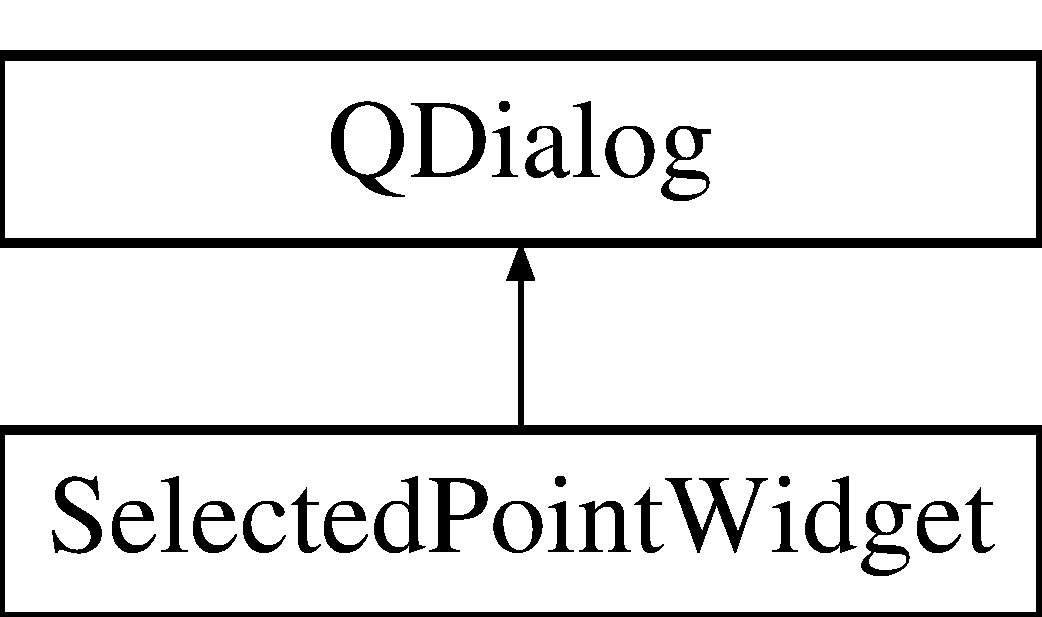
\includegraphics[height=2.000000cm]{class_selected_point_widget}
\end{center}
\end{figure}
\subsection*{Public Member Functions}
\begin{DoxyCompactItemize}
\item 
\hyperlink{class_selected_point_widget_a6973c27e249b2956b820cc67d8e01353}{Selected\+Point\+Widget} (vtk\+Smart\+Pointer$<$ vtk\+Poly\+Data $>$ points\+\_\+polydata, vtk\+Smart\+Pointer$<$ vtk\+Poly\+Data $>$ selected\+\_\+points\+\_\+polydata)
\item 
void \hyperlink{class_selected_point_widget_afd1322240157289461a8e97b744519c5}{populate} ()
\end{DoxyCompactItemize}
\subsection*{Public Attributes}
\begin{DoxyCompactItemize}
\item 
Q\+Table\+Widget $\ast$ {\bfseries table}\hypertarget{class_selected_point_widget_af975e399fc7a609981722bda4dbeea28}{}\label{class_selected_point_widget_af975e399fc7a609981722bda4dbeea28}

\item 
Q\+H\+Box\+Layout $\ast$ {\bfseries layout}\hypertarget{class_selected_point_widget_a9bc3e002ad38008034fa18e34c136e32}{}\label{class_selected_point_widget_a9bc3e002ad38008034fa18e34c136e32}

\item 
Q\+V\+Box\+Layout $\ast$ {\bfseries list\+\_\+holder\+\_\+layout}\hypertarget{class_selected_point_widget_a6305deed174162dbddab977db14bcc28}{}\label{class_selected_point_widget_a6305deed174162dbddab977db14bcc28}

\item 
Q\+Dialog\+Button\+Box $\ast$ {\bfseries button\+\_\+box}\hypertarget{class_selected_point_widget_aad58e8b55b796c4c60ec77e60ec70c5d}{}\label{class_selected_point_widget_aad58e8b55b796c4c60ec77e60ec70c5d}

\item 
Q\+Widget $\ast$ {\bfseries list\+\_\+holder\+\_\+widget}\hypertarget{class_selected_point_widget_a16b8e10427ac123e0d0a218a20b708a7}{}\label{class_selected_point_widget_a16b8e10427ac123e0d0a218a20b708a7}

\item 
Q\+Label $\ast$ {\bfseries transform\+\_\+direction\+\_\+title}\hypertarget{class_selected_point_widget_a69ea9e8a79fd9f1b508742b9ad71ef87}{}\label{class_selected_point_widget_a69ea9e8a79fd9f1b508742b9ad71ef87}

\item 
Q\+Label $\ast$ {\bfseries interpolation\+\_\+type\+\_\+title}\hypertarget{class_selected_point_widget_a8f260244a3198fa2e5d1d52dea031ae5}{}\label{class_selected_point_widget_a8f260244a3198fa2e5d1d52dea031ae5}

\item 
Q\+Combo\+Box $\ast$ {\bfseries transform\+\_\+direction\+\_\+list}\hypertarget{class_selected_point_widget_a08e55d0422a889983c7d4ba36d322f68}{}\label{class_selected_point_widget_a08e55d0422a889983c7d4ba36d322f68}

\item 
Q\+Combo\+Box $\ast$ {\bfseries interpolation\+\_\+type\+\_\+list}\hypertarget{class_selected_point_widget_a55451a9a8351fa26bffd964d20422edc}{}\label{class_selected_point_widget_a55451a9a8351fa26bffd964d20422edc}

\end{DoxyCompactItemize}


\subsection{Detailed Description}
Declaration of the \hyperlink{class_selected_point_widget}{Selected\+Point\+Widget} class. \hyperlink{class_selected_point_widget}{Selected\+Point\+Widget} refers to the widget displayed on the screen when the user selects at least one vertex of the displayed shape model by means of the rectangular box selector. The widget that is then displayed lists the I\+Ds of the selected vertices, as well as a choice of possible geometric transforms to be applied to them N\+O\+TE\+: for now, the only possible transform (homothetic transform) is hardcoded 

\subsection{Constructor \& Destructor Documentation}
\index{Selected\+Point\+Widget@{Selected\+Point\+Widget}!Selected\+Point\+Widget@{Selected\+Point\+Widget}}
\index{Selected\+Point\+Widget@{Selected\+Point\+Widget}!Selected\+Point\+Widget@{Selected\+Point\+Widget}}
\subsubsection[{\texorpdfstring{Selected\+Point\+Widget(vtk\+Smart\+Pointer$<$ vtk\+Poly\+Data $>$ points\+\_\+polydata, vtk\+Smart\+Pointer$<$ vtk\+Poly\+Data $>$ selected\+\_\+points\+\_\+polydata)}{SelectedPointWidget(vtkSmartPointer< vtkPolyData > points_polydata, vtkSmartPointer< vtkPolyData > selected_points_polydata)}}]{\setlength{\rightskip}{0pt plus 5cm}Selected\+Point\+Widget\+::\+Selected\+Point\+Widget (
\begin{DoxyParamCaption}
\item[{vtk\+Smart\+Pointer$<$ vtk\+Poly\+Data $>$}]{points\+\_\+polydata, }
\item[{vtk\+Smart\+Pointer$<$ vtk\+Poly\+Data $>$}]{selected\+\_\+points\+\_\+polydata}
\end{DoxyParamCaption}
)}\hypertarget{class_selected_point_widget_a6973c27e249b2956b820cc67d8e01353}{}\label{class_selected_point_widget_a6973c27e249b2956b820cc67d8e01353}
Constructor. The pointer passed as arguments allow the widget to have access to the point properties 
\begin{DoxyParams}{Parameters}
{\em points\+\_\+polydata} & Pointer to the vtk\+Poly\+Data storing the vertices of the shape model \\
\hline
{\em selected\+\_\+points\+\_\+polydata} & Pointer to the vtk\+Poly\+Data storing the selected vertices of the displayed shape model \\
\hline
\end{DoxyParams}


\subsection{Member Function Documentation}
\index{Selected\+Point\+Widget@{Selected\+Point\+Widget}!populate@{populate}}
\index{populate@{populate}!Selected\+Point\+Widget@{Selected\+Point\+Widget}}
\subsubsection[{\texorpdfstring{populate()}{populate()}}]{\setlength{\rightskip}{0pt plus 5cm}void Selected\+Point\+Widget\+::populate (
\begin{DoxyParamCaption}
{}
\end{DoxyParamCaption}
)}\hypertarget{class_selected_point_widget_afd1322240157289461a8e97b744519c5}{}\label{class_selected_point_widget_afd1322240157289461a8e97b744519c5}
Populates the Q\+Table\+Widget table with the relevant data 

The documentation for this class was generated from the following files\+:\begin{DoxyCompactItemize}
\item 
pdart\+\_\+prototype/source/selectedpointwidget.\+h\item 
pdart\+\_\+prototype/source/selectedpointwidget.\+cpp\end{DoxyCompactItemize}

%--- End generated contents ---

% Index
\backmatter
\newpage
\phantomsection
\clearemptydoublepage
\addcontentsline{toc}{chapter}{Index}
\printindex

\end{document}
